\documentclass[12pt]{article}
\usepackage{graphicx}

\usepackage{amsmath, amssymb}
\usepackage{enumitem}
\usepackage{geometry}
\geometry{margin=1in}

\newcommand{\myvec}[1]{\begin{bmatrix}#1\end{bmatrix}}
\newcommand{\brak}[1]{\left( #1 \right)}


\begin{document}

\begin{center}
    {\LARGE \textbf{GATE -2011 MT}} \\
    \vspace{1em}
    ai25btech11009 \qquad Dasu Harshith Kumar
\end{center}

\section*{Q.1 -- Q.25: One mark each}

\begin{enumerate}

\item Which one of the following methods is NOT used for numerically solving an ordinary differential equation (ODE)(GATE 2011 MT):
    \begin{enumerate}
        \item Euler's method
        \item Runge-Kutta method
        \item Adam-Bashforth method
        \item Newton-Raphson method
    \end{enumerate}

\item If two systems P and Q are in thermal equilibrium with a third system M, then P and Q will also be in thermal equilibrium with each other. This is following(GATE 2011 MT):
    \begin{enumerate}
        \item First law of Thermodynamics
        \item Second law of Thermodynamics
        \item Third law of Thermodynamics
        \item Zeroeth law of Thermodynamics
    \end{enumerate}

\item Humidification of the blast in the iron blast furnace leads to(GATE 2011 MT):
    \begin{enumerate}
        \item lowering of the raceway temperature
        \item increase in raceway temperature
        \item difficulty in pulverized coal injection (PCI)
        \item decrease of the oxygen content in the hot metal
    \end{enumerate}

\item Which one of the following refractory materials is NOT used in the BOF (LD) working lining(GATE 2011 MT)?
    \begin{enumerate}
        \item Tar-bonded dolomite
        \item Pitch-bonded magnesite
        \item Fired and pitch-impregnated magnesite
        \item Graphite-alumina composite
    \end{enumerate}

\item In the eutectoid steel, which one of the following structures DOES NOT form during continuous cooling(GATE 2011 MT)?
    \begin{enumerate}
        \item Fully pearlitic
        \item Pearlitic + bainitic
        \item Fully bainitic
        \item Martensitic
    \end{enumerate}

\item Which one of the following is a ferrite stabilizer in steels(GATE 2011 MT)?
    \begin{enumerate}
        \item Ni
        \item Cu
        \item Cr
        \item Mn
    \end{enumerate}

\item The angle between the line vector and the Burgers vector of an edge dislocation is(GATE 2011 MT):
    \begin{enumerate}
        \item 0 degree
        \item 90 degrees
        \item 120 degrees
        \item 180 degrees
    \end{enumerate}

\item In fracture toughness characterized by $K_{IC}$ or $J_{IC}$, I in the subscript indicates loading by(GATE 2011 MT):
    \begin{enumerate}
        \item crack opening mode
        \item forward shear mode
        \item parallel shear mode
        \item perpendicular shear mode
    \end{enumerate}

\item In a brazing process the liquid metal fills the gap by which one of the following means(GATE 2011 MT)?
    \begin{enumerate}
        \item Capillary infiltration
        \item Gravity infiltration
        \item Pressure infiltration
        \item Vacuum infiltration
    \end{enumerate}

\item Which one of the following expands upon solidification(GATE 2011 MT)?
    \begin{enumerate}
        \item Low carbon steel
        \item High carbon steel
        \item White cast iron
        \item Gray cast iron
    \end{enumerate}

\item For a simple cubic unit cell with unit vectors $i$, $j$, and $k$, the angle between lattice vectors [100] and  in degrees is(GATE 2011 MT):
    \begin{enumerate}
        \item 35.2
        \item 54.7
        \item 60
        \item 90
    \end{enumerate}

\item The inflection point of a nonlinear function $U(r)$ is at(GATE 2011 MT):
    \begin{enumerate}
        \item $U = 0$
        \item $\ln U = 0$
        \item $\frac{dU}{dr} = 0$
        \item $\frac{d^2U}{dr^2} = 0$
    \end{enumerate}

\item One mole of element P is mixed with one mole of element Q. The entropy of mixing at 0 K is(GATE 2011 MT):
    \begin{enumerate}
        \item 0
        \item $-R \ln 0.5$
        \item infinity
        \item $-R \ln 2$
    \end{enumerate}

\item Zinc rod is immersed in dilute HCl (pure). If a very small amount of FeCl$_3$ is added to the solution, the corrosion rate of zinc(GATE 2011 MT):
    \begin{enumerate}
        \item decreases
        \item increases
        \item remains constant
        \item is zero (passivation)
    \end{enumerate}

\item A metal is electrochemically polarized to a potential which is higher than the standard reduction potential of the metal. The overvoltage will be(GATE 2011 MT):
    \begin{enumerate}
        \item zero
        \item negative
        \item positive
        \item initially negative, then positive
    \end{enumerate}

\item Aluminum is NOT commercially produced by carbo-thermic reduction primarily because(GATE 2011 MT):
    \begin{enumerate}
        \item aluminum metal will have excessive dissolved oxygen
        \item it melts at too low a temperature
        \item it does not vaporize at reasonable temperatures
        \item Al-Al$_2$O$_3$ line is too low in the Ellingham diagram and needs excessively high temperatures
    \end{enumerate}

\item VOD process is preferred over AOD process for making extra-low carbon stainless steels because(GATE 2011 MT):
    \begin{enumerate}
        \item $p_{CO}$ can be lowered to a much lower level in the VOD than in the AOD
        \item AOD does not have adequate stirring
        \item free-board needed for such operation is not available in the AOD
        \item AOD refractory is not stable in contact with extra low carbon steel
    \end{enumerate}

\item In froth flotation, collector refers to a reagent which primarily(GATE 2011 MT):
    \begin{enumerate}
        \item promotes bubble break-up and stabilizes the foam
        \item adsorbs on the surface of the mineral, and makes it hydrophobic
        \item promotes separation of the particles from the froth
        \item absorbs on the unwanted mineral and makes it sink
    \end{enumerate}

\item With the increase in the degree of supercooling, the growth rate of a nucleus follows which one of the following trends(GATE 2011 MT)?
    \begin{enumerate}
        \item First increases and then decreases
        \item First decreases and then increases
        \item Only increases
        \item Only decreases
    \end{enumerate}

\item For a fcc unit cell, the ratio of the number of tetrahedral voids to the number of atoms is(GATE 2011 MT):
    \begin{enumerate}
        \item 2:1
        \item 3:1
        \item 4:1
        \item 5:1
    \end{enumerate}

\item The material in which there is conduction primarily by holes is(GATE 2011 MT):
    \begin{enumerate}
        \item conductor
        \item insulator
        \item p-type semiconductor
        \item n-type semiconductor
    \end{enumerate}

\item When load is applied to a material, 'instantaneous' strain develops with(GATE 2011 MT):
    \begin{enumerate}
        \item the speed of light
        \item half the speed of light
        \item the speed of sound
        \item infinite speed
    \end{enumerate}

\item For a given ductile material, which one of the following tensile properties obtained with non-standard specimen is NOT comparable to that obtained with standard specimen(GATE 2011 MT)?
    \begin{enumerate}
        \item Elongation to fracture
        \item Tensile strength
        \item Uniform elongation
        \item Yield strength
    \end{enumerate}

\item The nature of submerged arc welding flux with basicity index of 0.5 is(GATE 2011 MT):
    \begin{enumerate}
        \item neutral
        \item basic
        \item semi-basic
        \item acidic
    \end{enumerate}

\item Which one of the following carbon equivalent in steel is considered good for weldability(GATE 2011 MT)?
    \begin{enumerate}
        \item 1.0
        \item 0.8
        \item 0.6
        \item 0.4
    \end{enumerate}


% Q26
\item A box contains 5 white balls and 3 red balls. Two balls are withdrawn from the box randomly, one after another (without replacement). The probability that the two balls withdrawn are of different color is(GATE 2011 MT)
    \begin{enumerate}
        \item \(\frac{15}{64}\)
        \item \(\frac{25}{64}\)
        \item \(\frac{25}{56}\)
        \item \(\frac{30}{56}\)
    \end{enumerate}
% Q27
\item For a reaction \(A\rightarrow B\), if the rate of change in concentration of A (\(C_A\)), can be written as
\begin{align*}
\frac{dC_A}{dt} = kC_A^2
\end{align*}
then the change in concentration with time from initial concentration of A, \(C_{A0}\), is given by(GATE 2011 MT)
    \begin{enumerate}
        \item \((\frac{1}{C_A} - \frac{1}{C_{A0}}) = kt\)
        \item \((C_{A0} - C_A) = kt\)
        \item \((C_{A0} - C_A^2) = kt\)
        \item \(\ln(\frac{C_{A0}}{C_A}) = kt\)
    \end{enumerate}
% Q28
\item \(Y = k_1 - \exp{\left(\frac{k_2AX}{k_3X}\right)}\), where \(k_1, k_2, k_3\) are constants. If \(k_2AX \ll k_3X\), the value of Y up to first order of approximation would be(GATE 2011 MT)
    \begin{enumerate}
        \item \(Y = k_1 + \frac{k_2AX}{k_3X}\)
        \item \(Y = k_1\)
        \item \(Y = -k_1\)
        \item \(Y = k_1 - \frac{k_2AX}{k_3X}\)
    \end{enumerate}
% Q29
\item A large set of data for a given measurement is normally distributed around a mean \(\mu\), with standard deviation \(\sigma\). Which of the following limits would have about 95% of the data points around the mean and rest outside?(GATE 2011 MT)
    \begin{enumerate}
        \item \(\mu - 0.5\sigma\) and \(\mu + 0.5\sigma\)
        \item \(\mu - \sigma\) and \(\mu + \sigma\)
        \item \(\mu - 2\sigma\) and \(\mu + 2\sigma\)
        \item \(\mu - 3\sigma\) and \(\mu + 3\sigma\)
    \end{enumerate}
% Q30
\item During fully developed laminar flow in a circular pipe, the velocity profile is parabolic and symmetric around the axis. The velocity at the tube wall is zero. The ratio of the average velocity to the maximum velocity is(GATE 2011 MT)
    \begin{enumerate}
        \item \(\frac{1}{3}\)
        \item \(\frac{1}{2}\)
        \item \(\frac{2}{3}\)
        \item \(\frac{3}{4}\)
    \end{enumerate}
% Q31
\item If $k$ is the rate constant for a reaction and $T$ is the absolute temperature as in the figure, the activation energy for the reaction is(GATE 2011 MT)

\begin{center}
    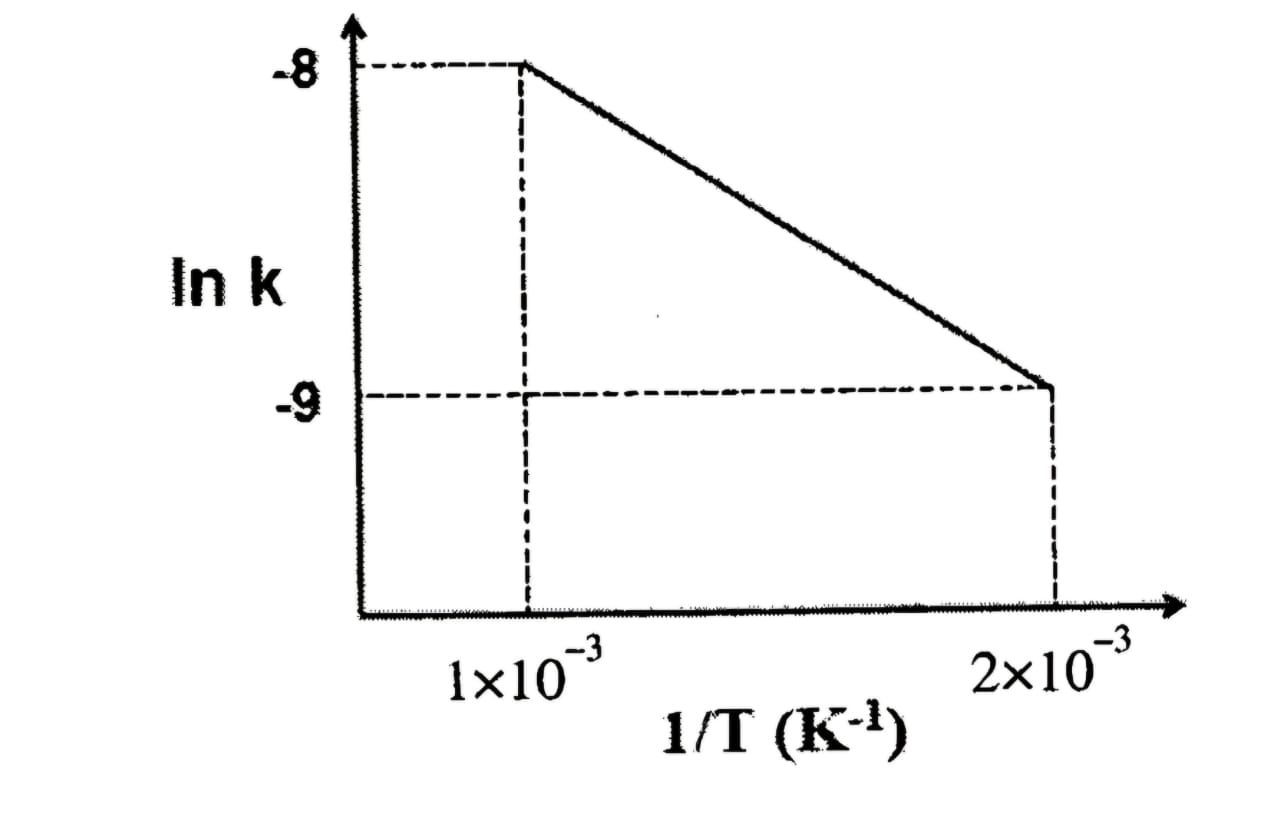
\includegraphics[width=0.6\textwidth]{images/q31image.jpg}
\end{center}

\begin{enumerate}
    \item 1,000 J/mol
    \item 2,000 J/mol
    \item 4,155 J/mol
    \item 8,314 J/mol
\end{enumerate}

% Q32
\item 
\begin{align*}
\text{2Cu(s) + 0.5O}_2(g) = \text{Cu}_2O(s) & : \Delta G^0 = -162200 + 69.24T \text{ J} \\
\text{2Cu(l) + 0.5O}_2(g) = \text{Cu}_2O(s) & : \Delta G^0 = -188300 + 88.48T \text{ J}
\end{align*}
The molar free energy change at 1300 K for transformation of solid Cu to liquid Cu will be(GATE 2011 MT)
    \begin{enumerate}
        \item 1,050 J
        \item 960 J
        \item 544 J
        \item 445 J
    \end{enumerate}
% Q33
\item 
\begin{align*}
\text{Al}_2O_3 + 6H^+ + 6e^- = 3H_2O + 2Al \\
\Delta G^0 = 897.3 \text{ kJ}
\end{align*}
The reduction potential of the above reaction under standard state will be(GATE 2011 MT)
    \begin{enumerate}
        \item $-1.55$ V
        \item $-1.40$ V
        \item 1.65 V
        \item 1.75 V
    \end{enumerate}
% Q34
\item \(G = U + PV - TS\). Then which one of the following is CORRECT?(GATE 2011 MT)
    \begin{enumerate}
        \item \((\frac{\partial V}{\partial T})_P = (\frac{\partial S}{\partial P})_T\)
        \item \((\frac{\partial V}{\partial T})_P = -(\frac{\partial S}{\partial P})_T\)
        \item \((\frac{\partial V}{\partial T})_P = (\frac{\partial P}{\partial S})_T\)
        \item \((\frac{\partial V}{\partial T})_P = -(\frac{\partial P}{\partial S})_T\)
    \end{enumerate}

% Q35 MATCHING TYPE
\item Match the metals in Group I with the corresponding ores in Group II.
\begin{table}[h]
\centering
\caption{Metal-Ore Matching}
\begin{tabular}{|c|c|c|}
\hline
\textbf{Group I (Metals)} & & \textbf{Group II (Ores)} \\
\hline
P. Lead & 3 & Galena \\
Q. Zinc & 5 & Sphalerite \\
R. Uranium & 4 & Pitchblende \\
S. Niobium & 1 & Columbite \\
\hline
\end{tabular}
\end{table}
\begin{enumerate}[label=(\Alph*)]
    \item P-3, Q-5, R-2, S-4
    \item P-3, Q-2, R-5, S-4
    \item P-3, Q-5, R-4, S-1
    \item P-3, Q-4, R-5, S-2
\end{enumerate}

% Q36
\item For the following reactions, the standard free energy change is given at 1773 K as follows(GATE 2011 MT):
\begin{align*}
\frac{2}{3} Cr_2O_3 (s) = \frac{4}{3} Cr (s) + O_2 (g) : \Delta G^0 = 447,800 \text{ J} \\
2 H_2 (g) + O_2 (g) = 2 H_2O (g) : \Delta G^0 = -297,000 \text{ J}
\end{align*}
If chromium oxide powder has to be reduced by hydrogen in a fluidized bed, the minimum $P_{H_2} / P_{H_2O}$ ratio that has to be maintained at the exit of the reactor is(GATE 2011 MT)
    \begin{enumerate}
        \item 8.5
        \item 10.6
        \item 100.2
        \item 166.5
    \end{enumerate}
% Q37
\item The hydrogen content of steel in equilibrium with hydrogen gas at 1 bar pressure is 28 ppm at some temperature. Hydrogen content in the metal at the same temperature gets reduced to 1 ppm, when the equilibrium $P_{H_2}$ changes to(GATE 2011 MT)
    \begin{enumerate}
        \item 28 bar
        \item $\frac{1}{28}$ bar
        \item $\left(\frac{1}{28}\right)^{0.5}$ bar
        \item $\left(\frac{1}{28}\right)^2$ bar
    \end{enumerate}
% Q38
\item A furnace wall consists of two layers. The inside layer of 450 mm is made of light weight bricks of thermal conductivity 1 W/m.K and the outside layer of 900 mm is made of refractory of thermal conductivity 2 W/m.K. The hot face of the inside layer is at temperature 1300 K and the cold face of the outer layer is at 400 K. The temperature at the interface between the two layers is (GATE 2011 MT)
    \begin{enumerate}
        \item 1000 K
        \item 850 K
        \item 700 K
        \item 600 K
    \end{enumerate}
% Q39 MATCHING TYPE
\item Match the heat treatment processes in Group I with resultant microstructure of steel in Group II.
\begin{table}[h]
\centering
\caption{Heat Treatment-Microstructure Matching}
\begin{tabular}{|c|c|c|}
\hline
\textbf{Group I} & & \textbf{Group II} \\
\hline
P. Martempering & 3 & Tempered martensite \\
Q. Normalising & 2 & Fine Pearlite \\
R. Subcritical annealing for long time & 4 & Spheroidised cementite in matrix of ferrite \\
S. Full annealing & 1 & Coarse Pearlite \\
\hline
\end{tabular}
\end{table}
\begin{enumerate}[label=(\Alph*)]
    \item P-1, Q-4, R-3, S-2
    \item P-2, Q-3, R-1, S-4
    \item P-4, Q-1, R-2, S-3
    \item P-3, Q-2, R-4, S-1
\end{enumerate}
% Q40
\item In case of homogeneous nucleation, the critical edge length for a cube shaped nucleus is $(\gamma$: Energy per unit area of the interface between the product and parent phase; $\Delta g$: Gibbs free energy change per unit volume)(GATE 2011 MT)
    \begin{enumerate}
        \item $-4\gamma/\Delta g$
        \item $-2\gamma/\Delta g$
        \item $\gamma/\Delta g$
        \item $-3\gamma/\Delta g$
    \end{enumerate}
% Q41
\item For a cubic metal with lattice parameter of 3.92 Å, the first four diffraction peaks from the X-ray powder diffraction pattern taken with CuK$\alpha$ radiation $(\lambda = 1.5405\, \text{\AA})$ occur at $2\theta$ values of 39.7, 46.2, 67.5, and 81.3 degrees. The crystal structure of the metal is (GATE 2011 MT)
    \begin{enumerate}
        \item simple cubic
        \item fcc
        \item bcc
        \item diamond cubic
    \end{enumerate}
% Q42
\item The largest size of immobilized segment of dislocation in a Frank-Read (FR) source in a polycrystalline material is of the order of grain size. In a metal of 10 $\mu$m grain size, the shear stress required to operate such a FR source is 100 MPa. If the grain size is reduced to 10 nm, the shear stress required to operate such FR source would be (GATE 2011 MT)
    \begin{enumerate}
        \item $10^{2}$ MPa
        \item $10^{3}$ MPa
        \item $10^{5}$ MPa
        \item $10^{6}$ MPa
    \end{enumerate}
% Q43
\item Which one of the following reactions in fcc/bcc crystals with lattice parameter a is energetically favorable? (GATE 2011 MT)
    \begin{enumerate}
        \item $a/2 [110] + a/2  \to a/2 $
        \item $a/2  + a/2  \to a $
        \item $a/2  + a/2  \to a $
        \item $a/2  + a/2  \to a/2 $
    \end{enumerate}

% Q44 MATCHING TYPE: hardness test
\item Match the hardness test methods in Group I with the indenter used in Group II. (GATE 2011 MT)
\begin{table}[h]
\centering
\caption{Hardness Test-Indenter Matching}
\begin{tabular}{|c|c|c|}
\hline
\textbf{Group I} & & \textbf{Group II} \\
\hline
P. Brinell hardness & 3 & 10 mm diameter steel ball \\
Q. Vickers hardness & 2 & Square base diamond pyramid \\
R. Rockwell C hardness & 1 & Brale indenter \\
S. Rockwell B hardness & 4 & 1.6 mm diameter steel ball \\
\hline
\end{tabular}
\end{table}
\begin{enumerate}[label=(\Alph*)]
    \item P-1, Q-2, R-3, S-4
    \item P-3, Q-2, R-1, S-4
    \item P-1, Q-4, R-3, S-2
    \item P-1, Q-2, R-4, S-3
\end{enumerate}

% Q45 assertion-reason
\item Assertion 'a': During casting of aluminium, grain refinement can be achieved by addition of certain alloying elements. \\
Reason 'r': The addition of the alloying element may result in the formation of deoxidation products or intermetallic compounds which may act as nucleation sites for grain refinement.
    \begin{enumerate}
        \item Both 'a' and 'r' are true but 'r' is not the reason for 'a'
        \item Both 'a' and 'r' are true and 'r' is the reason for 'a'
        \item 'a' is true but 'r' is false
        \item 'a' is false but 'r' is true
    \end{enumerate}

% Q46 MATCHING TYPE
\item Match those listed in Group I with the NDT methods listed in Group II.(GATE 2011 MT)
\begin{table}[h]
\centering
\caption{NDT Method Matching}
\begin{tabular}{|c|c|c|}
\hline
\textbf{Group I} & & \textbf{Group II} \\
\hline
P. Penetrameter & 3 & X-Ray radiography \\
Q. Differential coil probe & 4 & Acoustic emission test \\
R. Piezo-electric probe & 1 & Ultrasonic test \\
S. Developer & 2 & Dye-penetrant test \\
\hline
\end{tabular}
\end{table}
\begin{enumerate}[label=(\Alph*)]
    \item P-3, Q-4, R-1, S-2
    \item P-2, Q-1, R-3, S-4
    \item P-1, Q-2, R-4, S-3
    \item P-4, Q-3, R-2, S-1
\end{enumerate}

% Q47 MATCHING TYPE
\item Match the manufacturing process of Group I to be used for producing the product in Group II. (GATE 2011 MT)
\begin{table}[h]
\centering
\caption{Process-Product Matching}
\begin{tabular}{|c|c|c|}
\hline
\textbf{Group I} & & \textbf{Group II} \\
\hline
P. Drawing & 2 & Tube \\
Q. Forging & 3 & Crank shaft \\
R. Rolling & 4 & Plate \\
S. Stretch forming & 1 & Large curved disc \\
\hline
\end{tabular}
\end{table}
\begin{enumerate}[label=(\Alph*)]
    \item P-2, Q-3, R-4, S-1
    \item P-1, Q-4, R-3, S-2
    \item P-3, Q-2, R-1, S-4
    \item P-4, Q-1, R-2, S-3
\end{enumerate}



% Q48
\item An aluminium billet of 300 mm diameter is extruded with an extrusion ratio of 16. What is the diameter of the final product? (GATE 2011 MT)
    \begin{enumerate}
        \item 150 mm
        \item 75 mm
        \item 59 mm
        \item 19 mm
    \end{enumerate}

% Q49
\item What is the ideal extrusion pressure if the effective flow stress in compression is 250 MPa? (GATE 2011 MT)
    \begin{enumerate}
        \item 693 MPa
        \item 346 MPa
        \item -346 MPa
        \item -703 MPa
    \end{enumerate}

% Q50
\item At the eutectoid point, the alloy has $\alpha$ and $\beta$ in the weight ratio 1:1. The eutectoid point occurs at composition (GATE 2011 MT)
    \begin{enumerate}
        \item 46 wt\% Q
        \item 47.5 wt\% Q
        \item 50 wt\% Q
        \item 52.5 wt\% Q
    \end{enumerate}

% Q51
\item At the eutectoid temperature, the ratio of $\alpha$ and $\beta$ phases in the specimen observed under microscope is (GATE 2011 MT)
    \begin{enumerate}
        \item 0.50
        \item 0.40
        \item 0.25
        \item 0.20
    \end{enumerate}

% Q52
\item The amount of oxygen in CO and CO$_2$ leaving with the top gas is (GATE 2011 MT)
    \begin{enumerate}
        \item 293 kg
        \item 407 kg
        \item 700 kg
        \item 1050 kg
    \end{enumerate}

% Q53
\item The CO/CO$_2$ molar ratio in the top gas is (GATE 2011 MT)
    \begin{enumerate}
        \item 0.9
        \item 1.0
        \item 1.1
        \item 1.5
    \end{enumerate}

% Q54
\item The magnitude of Burgers vector in copper is (GATE 2011 MT)
    \begin{enumerate}
        \item 2.54~\AA
        \item 2.39~\AA
        \item 2.20~\AA
        \item 2.18~\AA
    \end{enumerate}

% Q55
\item The elastic strain energy per unit length of dislocation line in copper is (GATE 2011 MT)
    \begin{enumerate}
        \item 34.8 $\times 10^{-10}$~N
        \item 28.8 $\times 10^{-10}$~N
        \item 24.8 $\times 10^{-10}$~N
        \item 14.5 $\times 10^{-10}$~N
    \end{enumerate}

% Q56
\item Choose the word from the options given below that is most nearly opposite in meaning to the given word: Frequency (GATE 2011 MT)
    \begin{enumerate}
        \item periodicity
        \item rarity
        \item gradualness
        \item persistency
    \end{enumerate}

% Q57
\item Choose the most appropriate word from the options below to complete the sentence:
It was her view that the country's problems had been      by foreign technocrats, so that to invite them to come back would be counter-productive.(GATE 2011 MT)
    \begin{enumerate}
        \item identified
        \item ascertained
        \item exacerbated
        \item analysed
    \end{enumerate}

% Q58
\item There are two candidates P and Q in an election. During the campaign, 40\% of the voters promised to vote for P, and rest for Q. However, on the day of election 15\% of the voters went back on their promise to vote for P and voted for Q. 25\% of the voters went back on their promise to vote for Q and voted for P. Suppose, P lost by 2 votes, then what was the total number of voters? (GATE 2011 MT)
    \begin{enumerate}
        \item 100
        \item 110
        \item 90
        \item 95
    \end{enumerate}

% Q59
\item Gladiator: Arena
    \begin{enumerate}
        \item dancer: stage
        \item commuter: train
        \item teacher: classroom
        \item lawyer: courtroom
    \end{enumerate}

% Q60
\item Under ethical guidelines recently adopted by the Indian Medical Association, human genes are to be manipulated only to correct diseases for which     treatments are unsatisfactory. (GATE 2011 MT)
    \begin{enumerate}
        \item similar
        \item most
        \item uncommon
        \item available
    \end{enumerate}

% Q61
\item Given that $f(y) = \frac{|y|}{y}$, and $q$ is any non-zero real number, the value of $|f(q) - f(-q)|$ is (GATE 2011 MT)
    \begin{enumerate}
        \item 0
        \item -1
        \item 1
        \item 2
    \end{enumerate}

% Q62
\item Three friends, R, S and T shared toffee from a bowl. R took 1/3rd of the toffees, but returned four to the bowl. S took 1/4th of what was left but returned three toffees to the bowl. T took half of the remainder but returned two back into the bowl. If the bowl had 17 toffees left, how many toffees were originally there in the bowl? (GATE 2011 MT)
    \begin{enumerate}
        \item 38
        \item 31
        \item 48
        \item 41
    \end{enumerate}

% Q63 
\item The fuel consumed by a motorcycle during a journey at various speeds is indicated in the graph below. (GATE 2011 MT)

\begin{center}
    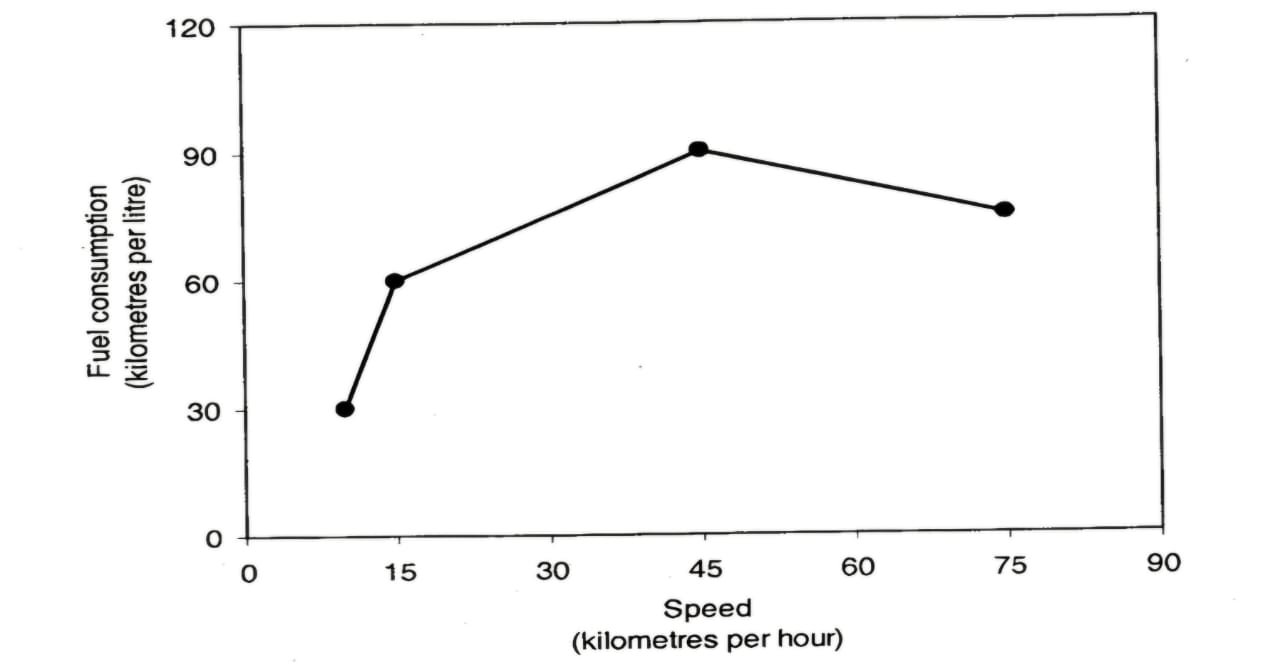
\includegraphics[width=0.6\textwidth]{images/q63image1.jpg}
\end{center}

The distances covered during four laps of the journey are listed in the table below.

\begin{center}
    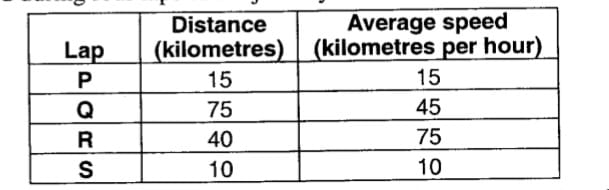
\includegraphics[width=0.8\textwidth]{images/q63image2.jpg}
\end{center}

From the given data, we can conclude that the fuel consumed per kilometre was least during the lap
    \begin{enumerate}
        \item P
        \item Q
        \item R
        \item S
    \end{enumerate}

% Q64
\item The horse has played a little known but very important role in the field of medicine. Horses were injected with toxins of diseases until their blood built up immunities. Then a serum was made from their blood. Serums to fight with diphtheria and tetanus were developed this way. 
It can be inferred from the passage, that horses were (GATE 2011 MT)
    \begin{enumerate}
        \item given immunity to diseases
        \item generally quite immune to diseases
        \item given medicines to fight toxins
        \item given diphtheria and tetanus serums
    \end{enumerate}

% Q65
\item The sum of $n$ terms of the series $4+44+444+\ldots$ is
    \begin{enumerate}
        \item $\frac{4}{81}[10^{n+1} - 9n - 1]$
        \item $\frac{4}{81}[10^{n-1} - 9n - 1]$
        \item $\frac{4}{81}[10^{n+1} - 9n - 10]$
        \item $\frac{4}{81}[10^n - 9n - 10]$
    \end{enumerate}

\end{enumerate}
\end{document}